\chapter{The Karas Pipeline}
\label{cha:karas-pipeline}

This chapter presents the GPU pipeline proposed by
\cite{karas2019data} (henceforth referred to as the \textit{Karas
  Pipeline} in more detail since the work presented in this report is
directly based off of this seminal work. The chapter concludes by
presenting the limitations of the Karas Pipeline and derives
motivations for a better alternative as presented in the following
chapters (see chapters \ref{cha:pm} and \ref{cha:gcd}).

Karas et al. presents a data processing pipeline to filter timeslices
containing hits from neutrino events from those containing only noise.
The pipeline is able to achieve this filtration by processing the data
in 3 steps, illustrated in Figure \ref{fig:karas-pipeline} and
described in more detail below. Figure \ref{fig:karas-pipeline-data}
provides a visual representation of the various shapes and
arrangements of the data as it passes through the pipeline.

\begin{figure}[h]
  \centering
  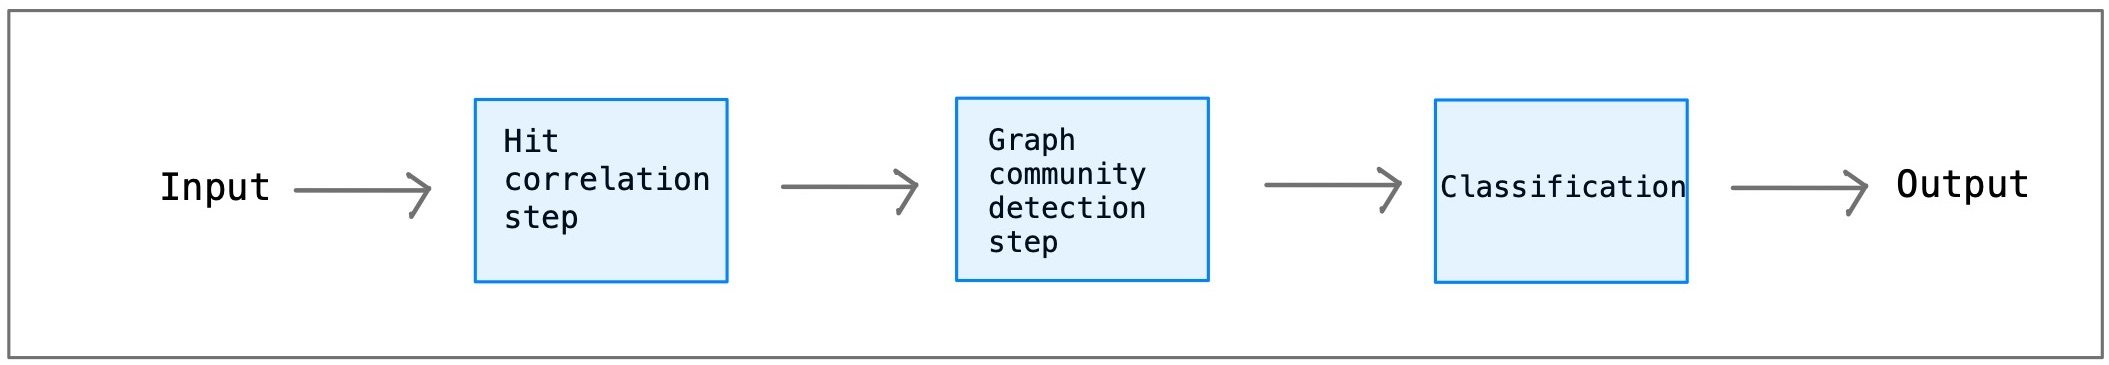
\includegraphics[width=\textwidth]{karas-pipeline.jpg}
  \caption{Overview of Karas Pipeline}
  \label{fig:karas-pipeline}
\end{figure}

\begin{figure}[h]
  \centering
  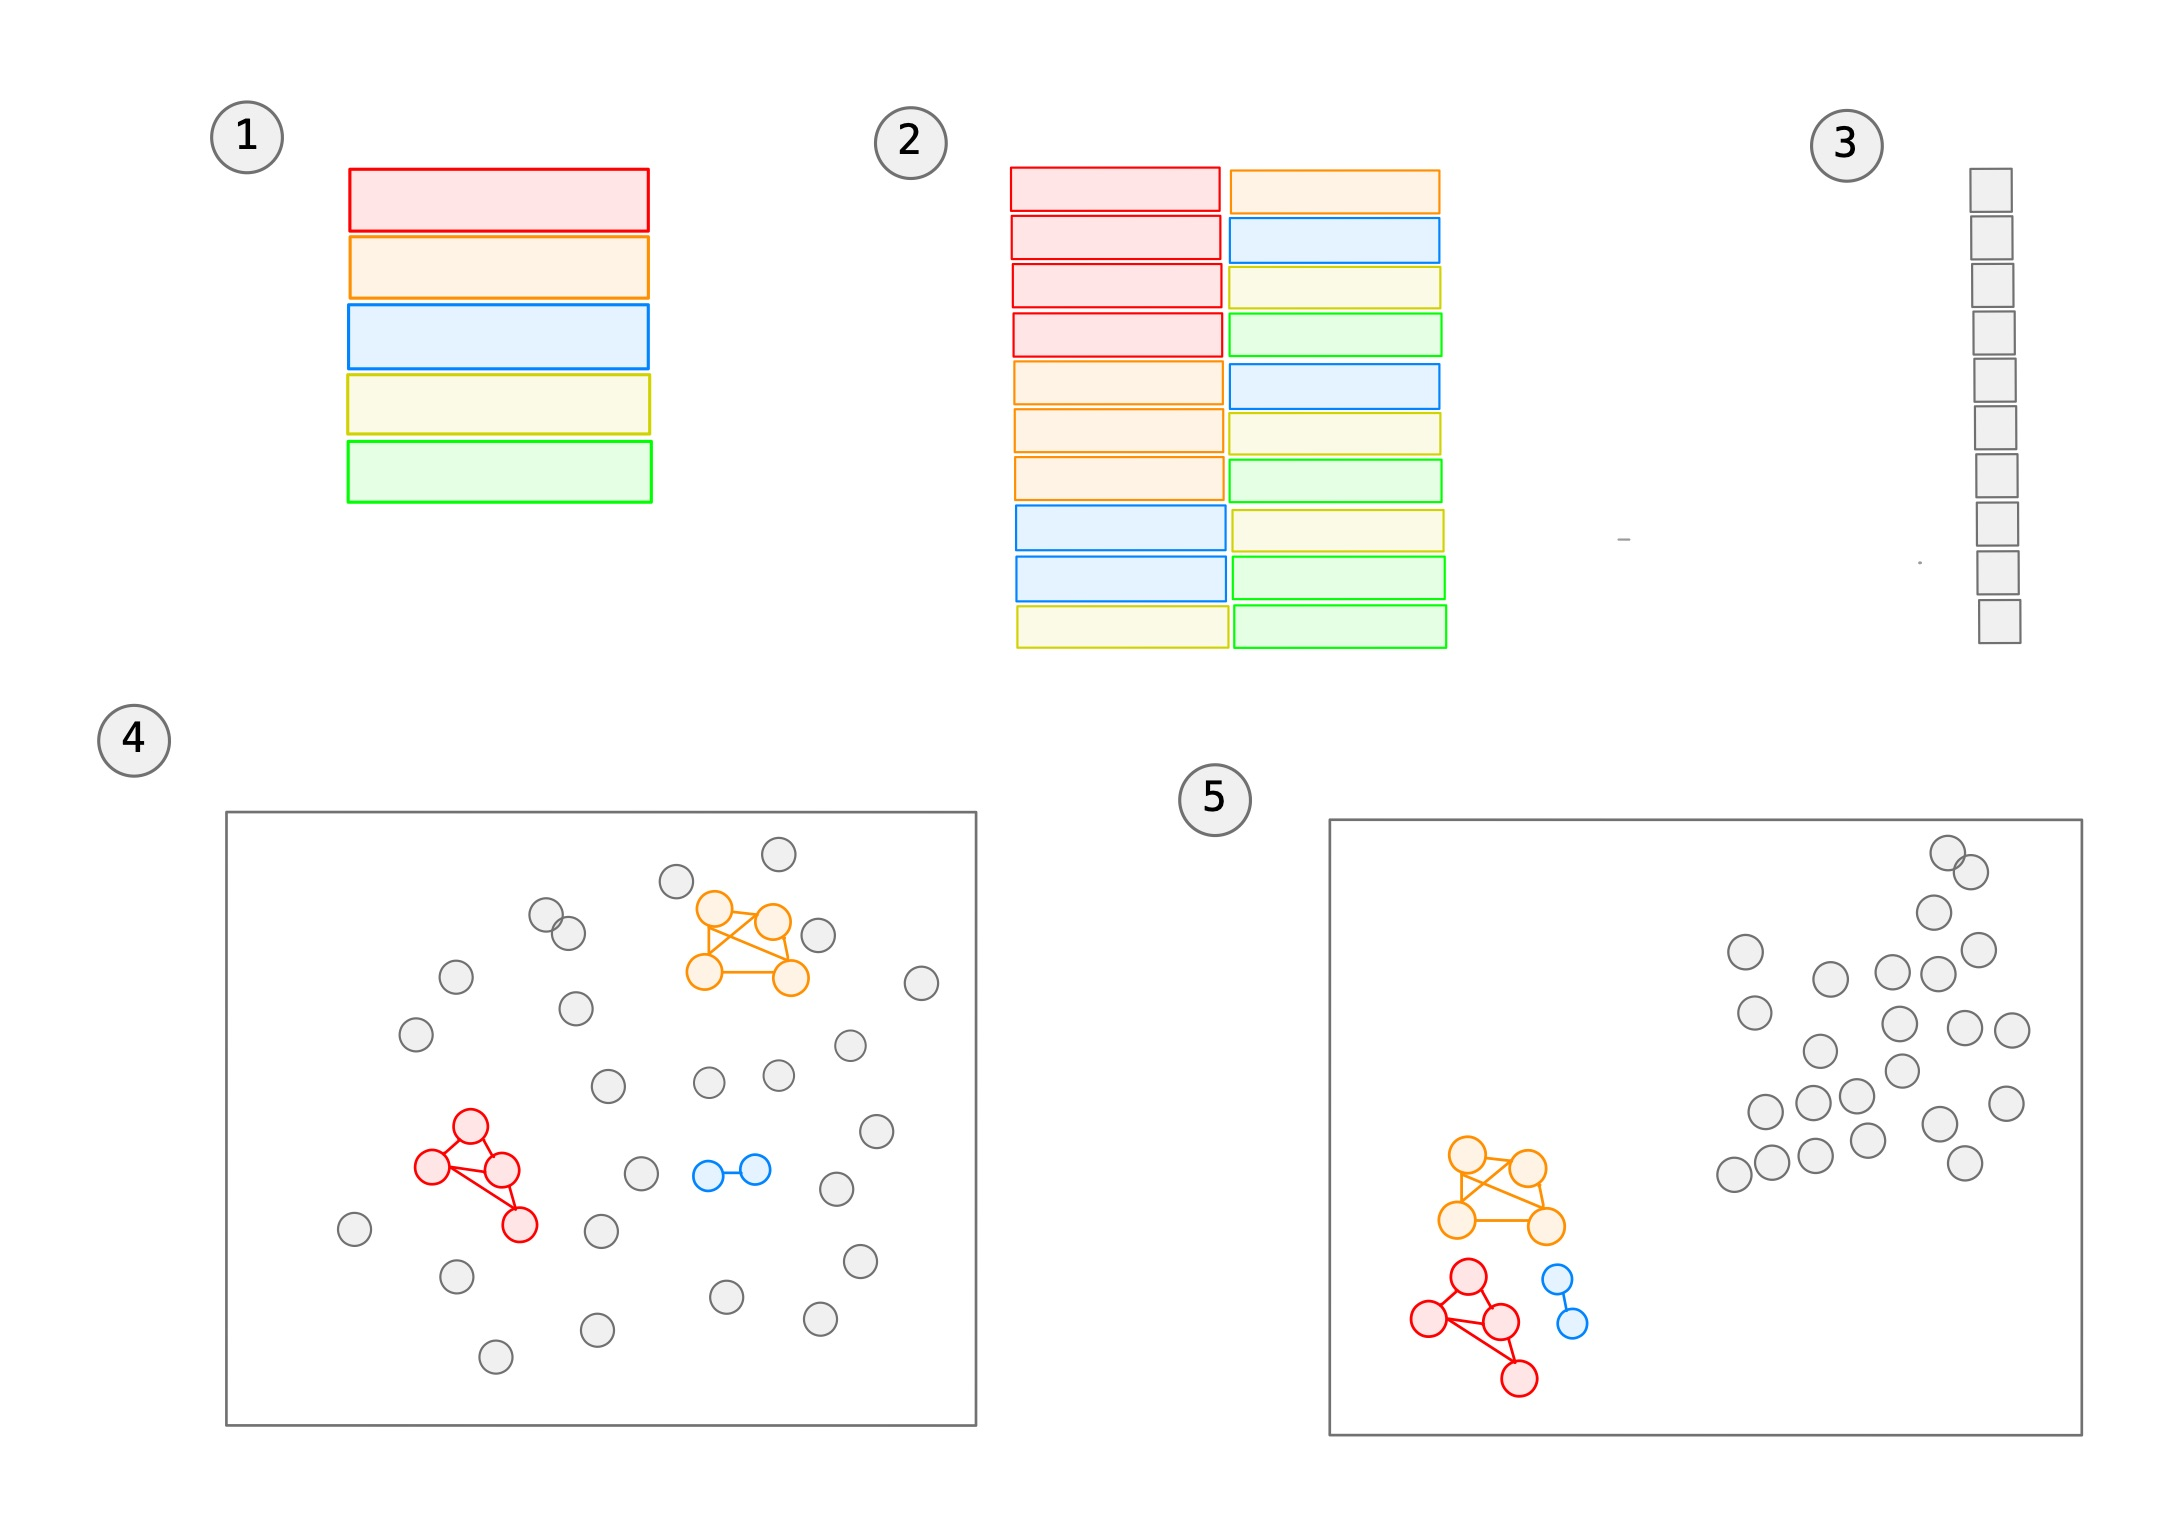
\includegraphics[width=\textwidth]{karas-pipeline-data.jpg}
  \caption{\textbf{(1)}. The main dataset of the project, each row
    representing a hit consisting of the $(x, y, z, t) vector$. Here
    an example set containing 5 hits is shown. \textbf{(2)}. The input
    to the Correlation Step is all unique pairs of hits. \textbf{(3)}.
    The output of the Correlation Step is a vector containing the
    probability that the pairs of hits are related to each other.
    \textbf{(4)}. (1) and (3) are used to construct a graph
    representation of the dataset where event (red, orange and blue)
    and noise (grey) hits are represented as nodes and related nodes
    are connected by an undirected edge carrying as weight the
    probability of being related. \textbf{(5)}. The graph from (4)
    acts as the input to the Graph Community Detection step, the
    output of which is another graph where event and noise nodes are
    grouped together and thus are linearly separable from each other.}
  \label{fig:karas-pipeline-data}
\end{figure}

The first step of The Karas pipeline is the Hit Correlation step which
proposes \emph{The Pattern Matrix Criterion (PMC)} to identify hits
which may have originated from the same neutrino event, referred to as
\emph{causally related} hits. From domain knowledge, it is known that
related hits occur close to each other both in space and time.
Specifically, the space and time difference of related hits is found
to be 100m and 300ns respectively. The PMC operates by creating a
correlation criterion based on the probability that the aforementioned
space and time difference occurs between two related hits. Pairs of
hits (from both events and noise) are passed to the PMC as input, the
output being an adjacency matrix where related hits are assigned a
high score whilst unrelated hits are assigned a lower score. The
algorithm is evaluated with a dataset containing 130 event hits and
5000 noise hits and scores in the range of 0.3 - 0.375 is reported for
the recall, precision and F1 metrics and an accuracy of 80\% is
achieved. Due to the stocastic nature of hits, unrelated hits such as
noise-event or noise-noise pairs may occur within this predefined
range thus being falsely identified as related. This is rectified in
the next step of the pipeline.

The second step of the Karas pipeline is the Graph Community Detection
(GCD) step. The main dataset is represented as a graph where hits are
represented as nodes. All nodes are connected with each other and
carry as weight the probability of being related using the output of
the PMC. The \emph{Constant Potts Model (CPM)} is used to group the
nodes into separate communities (or clusters) of related and unrelated
hits. The model is tested using a dataset consisting of 130 event hits
and 5000 noise hits and performs exceptionally well as it is able to
group most event hits into a single community and the noise in
another.

Since the GCD step directly operates on the data derived using the Hit
Correlation step, communities may still contain noise nodes. Thus the
third and final step of the pipeline classifies given communities as
\emph{event} or \emph{noise} communities based on the exclusive
presence of event nodes. This can be done by observing two properties
of the graph namely the size of the communities and the density of
edges within the communities. Communities consisting exclusively of
event nodes with be of small sizes and have high edge density whilst
communities consisting a mix of event and noise nodes or only noise
nodes will be relatively larger and have lesser edge density. The two
parameters which aid in the classification are the Probability
Threshold (PT) of the PMC and the CPM resolution parameter ($\gamma$)
of the GCD step. The PT and $\gamma$ are grid searched to determine
their optimal thresholds, all hits above the specified thresholds are
classified as event communities and the rest as noise communities.

\subsection{Limitations of the Karas Pipeline}
\label{sec:karas-pipeline-limitations}

Although The Karas Pipeline is able to identify timeslices with
neutrino event hits more accurately compared to its predecessors
\cite{karas2019data}, the pipeline still has certain limitations which
hinders its performance. To begin, the space and time difference based
on which the PMC determines if two hits are causally related to one
another is static. This may result in related hits which do not meet
these thresholds to be incorrectly given a low score. Due to the
stocastic nature of hits, event-noise and noise-noise pairs which fall
within the thresholds may also occur and these will be incorrectly
given a high score. The communities created created by CPM is biased
by the edge weights provided by the PMC. Furthermore, the
classification step also operates on static values of the PT and
$\gamma$ and thus is unable to identify communities of size smaller
than 20 hits.

Instead of deriving the correlation thresholds manually, a better
approach may be to use NNs to learn the optimal thresholds. This idea
is further explored in Chapter \ref{cha:mlp} where a MLP is used to
classify related and unrelated hits. Recently, the field of Geometric
Deep Learning has gained popularity which some very exciting
developments in models which are designed to operate upon graph
structures. Once such development is the Graph Convolusional Neural
(GCN) Network proposed by Kipf et al. The limitations of the GCD and
classification steps may be alleviated by using a GCN to classify
event and noise nodes and is explored in Chapter \ref{cha:gcn}.
